\documentclass[11pt,a4paper,english]{article}
\usepackage{babel}
\usepackage[utf8]{inputenc}
\usepackage{amsmath}
\DeclareMathOperator*{\argmax}{\arg\max}
\DeclareMathOperator*{\logit}{\text{logit}}
\usepackage{amsfonts}
\usepackage{amssymb}
\usepackage{graphicx}
\usepackage{natbib}
\usepackage{bbm}
\usepackage{tabularx,booktabs}
\newcommand\numberthis{\stepcounter{equation}{}\tag{Equation \theequation}}
\newcommand\iid{\mathrel{\overset{\makebox[0pt]{\mbox{\normalfont\tiny\sffamily i.i.d.}}}{\sim}}}


\newcolumntype{B}{>{\centering\arraybackslash}X}

\addtolength{\oddsidemargin}{-.895in}
	\addtolength{\evensidemargin}{-.895in}
	\addtolength{\textwidth}{1.75in}

\addtolength{\topmargin}{-1.25in}
	\addtolength{\textheight}{1.75in}

%\author{Joelle Mbatchou}
\title{On \texttt{predict.MCMCglmm}}
%\date{\vspace{-6ex}Oct. $9^{\text{th}}$ 2015}
\date{\vspace{-7ex}}
\begin{document}
\maketitle

%Given the covariates, genotypes and random effects ($X$, $W$ and $U$ respectively), we generate the binary trait $Y$ according to the following logistic mixed model
%\begin{align*}
%Y_i|\pi_i &\sim \text{Ber}(\pi_i),\\
%\text{logit}(\pi_i) &=  X_i^T\beta +\lambda \mathbbm{1}_{\{W_{1i}\,>\,0,W_{2i}\,>\,0\}} + U_i,\numberthis\\
% \mathbf{U} &\sim \; MVN(0, \sigma_a^2\, \Phi),
%\end{align*}
%where we include the genotype vectors of two causal unobserved common variants $\mathbf{W}_1$ and $\mathbf{W}_2$ (MAF is 0.1 and 0.2 respectively) coded as 0,1 or 2 (i.e. the minor allele count) and $\lambda$ denotes their epistatic effect on the phenotype. Its value corresponds to an increase of about 10\% in the penetrance for individuals that have at least one mutation at both causal loci compared to individuals that don't have any mutation at one (or both) of the two loci. The mean prevalence of the trait is 11\%. We also include three covariates that affect the trait: age, sex and a $N(0,1)$ covariate $\mathbf{Z}$. Families are ascertained based on having at least 5 affected members.

\begin{align*}
\text{{\bf Gen. model}:  }\logit(\pi_i) &=  \textbf{X}_i\,\boldsymbol{\beta} + \underbrace{G_i\gamma+ u_i},\numberthis\\
\text{{\bf Fitted model}:  }\logit(\pi_i) &= l_i =\textbf{X}_i\,\boldsymbol{\beta} +\,\;\quad u^*_i\;\quad, \numberthis
\end{align*}

\underline{Four estimates for $ \mathbf{u}^*$:}
\begin{enumerate}
\item Posterior mean of $ \mathbf{u}^*$
\item Posterior mode of $ \mathbf{u}^*$
\item Posterior mean of $ \mathbf{l} -\textbf{X}\,\boldsymbol{\beta}$
\item Posterior mode of $ \mathbf{l} -\textbf{X}\,\boldsymbol{\beta}$
\end{enumerate}

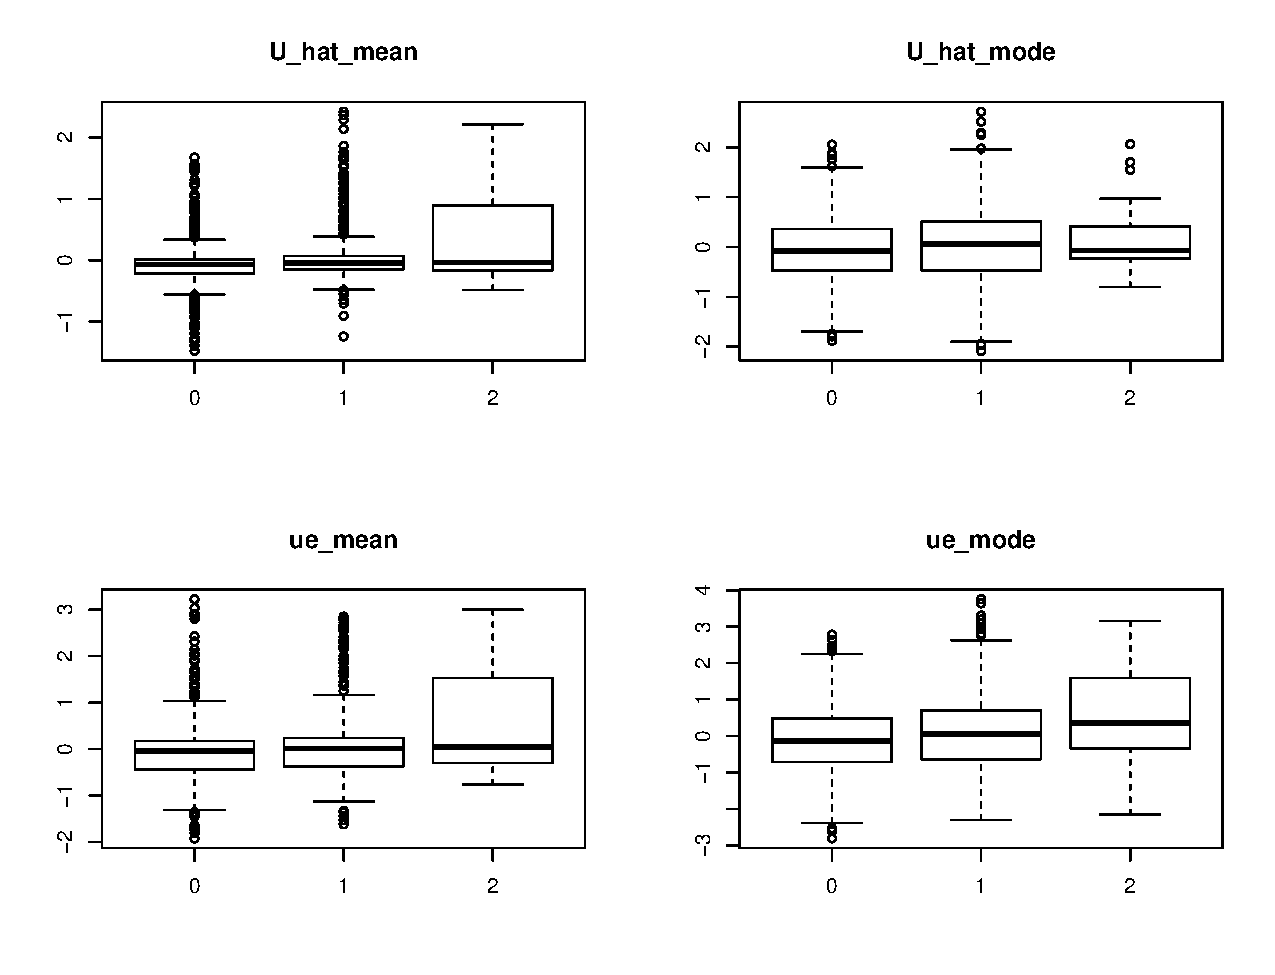
\includegraphics[page=1,scale=.4]{corGU2.pdf}
\includegraphics[page=2,scale=.4]{corGU2.pdf}\\
\begin{center}
\noindent\rule{8cm}{0.4pt}
\end{center}

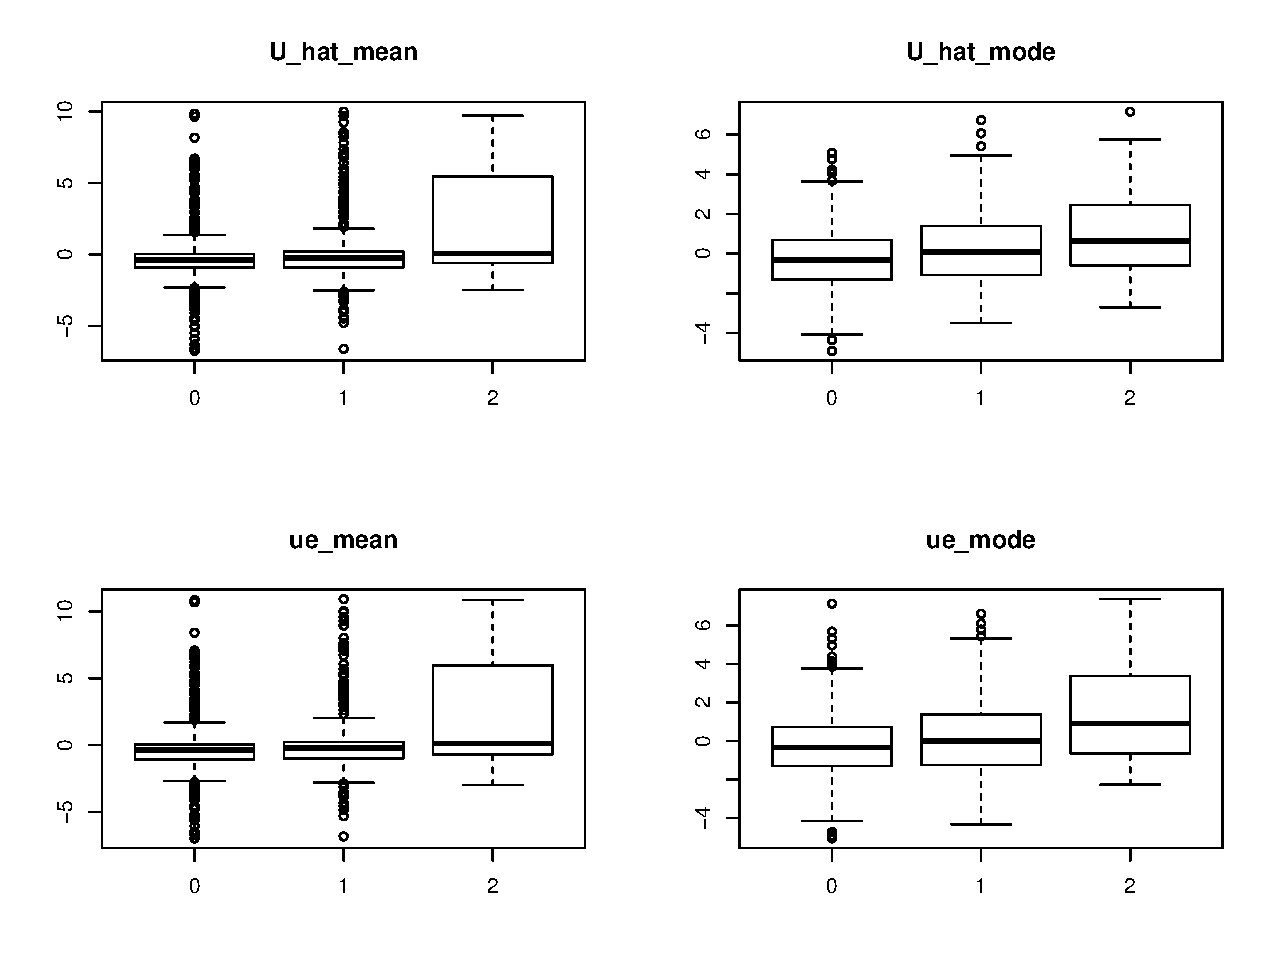
\includegraphics[page=1,scale=.4]{corGU3.pdf}
\includegraphics[page=2,scale=.4]{corGU3.pdf}\\


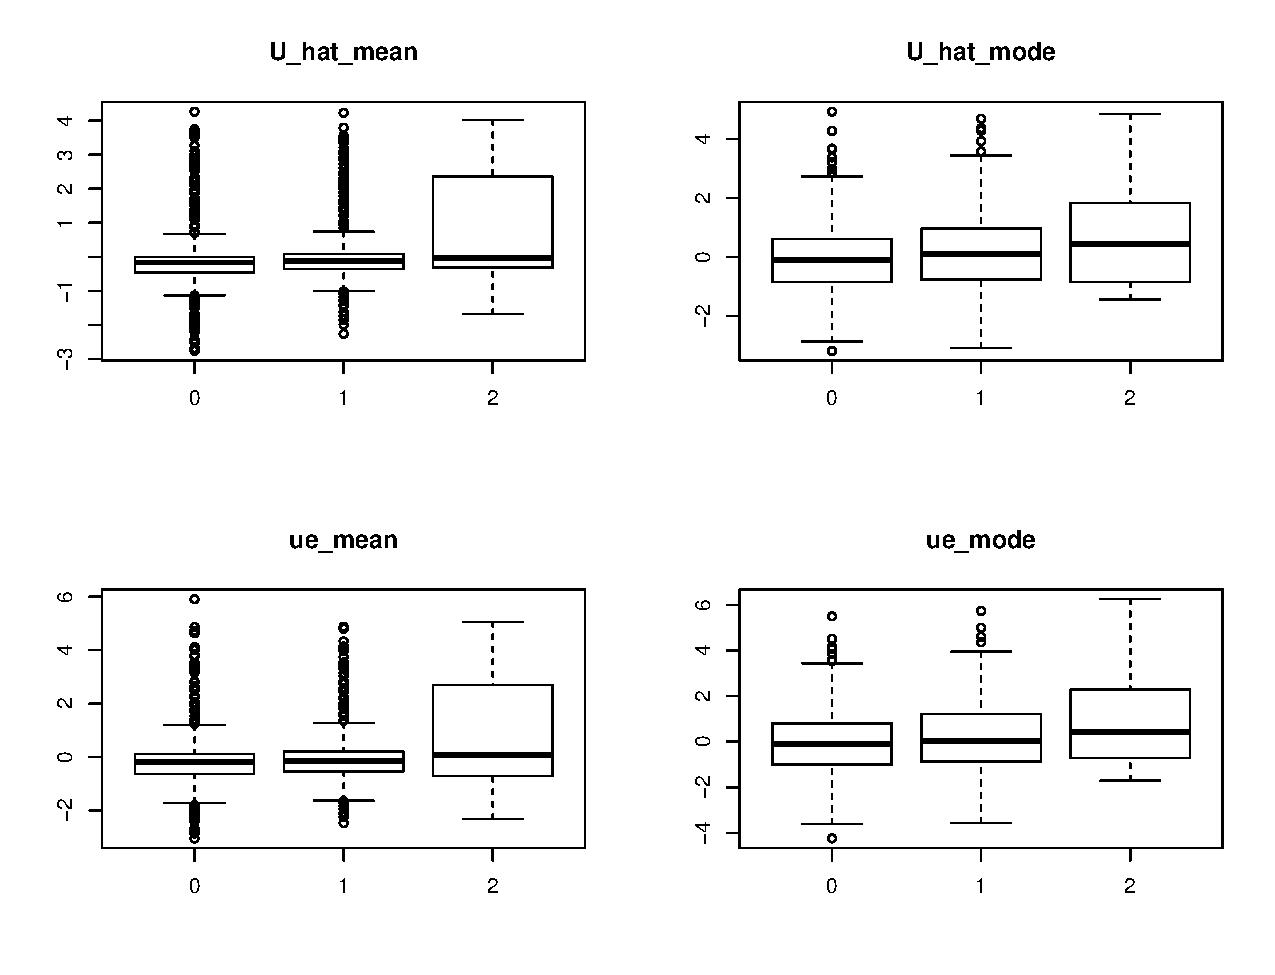
\includegraphics[page=1,scale=.4]{corGU5.pdf}
\includegraphics[page=2,scale=.4]{corGU5.pdf}\\
\end{document}

\noindent\rule{15cm}{0.4pt}

- Effective sample size is much bigger when ascertainment is present => b/c of much higher proportion of cases than in population? = better mixing??
	-> but mcmc estimates for the fixed effects are about the same
	
-- Why the error term is not identifiable in logistic model
First, let y* be the some unobserved latent/underlying variable, that is a linear function of some covariates and parameters, i.e.

               y* = x'β + σ ε ,                                                                             (1)

where ε follows some distribution, F(.), with E(ε) = 0.
If F(.) = Λ(.), the c.d.f. for the logistic distribution, then we get the Logit model.

What we actually observe is a value for an indicator variable, y, with:

            y = 1     if   y* > 0
            y = 0     if   y* ≤ 0 .                                                                       (2)

Note that we can re-write equation (1) as:

          ( y* / σ) = x' (β / σ) +  ε .                                                                 (3)

Then, notice that because the scale parameter σ must be positive, the sign of y* will be the same as that of ( y* / σ). So, regardless of whether we use (1) or (3), the observed variable, y, will take its zero-one values in exactly the same way. Therefore, the parameter σ cannot be identified in this model and so we may as well set it to 1.
